\section{Part A Discussion}

\subsection{a}
Kernel is the area that is scanned around a pixel. Lager amount of pixels surround the pixel of interest will be scanned for a larger kernel. If the kernel size increases, the image will become more blurred because the size corresponds to the standard deviation, $\sigma$, of Gaussian distribution. In other words, increasing kernel size decreases the weight of the pixels around centre and increases the weight of the distal pixels. This gives a blurrier image.



\subsection{b}
\begin{figure}[htbp]
   \centering
   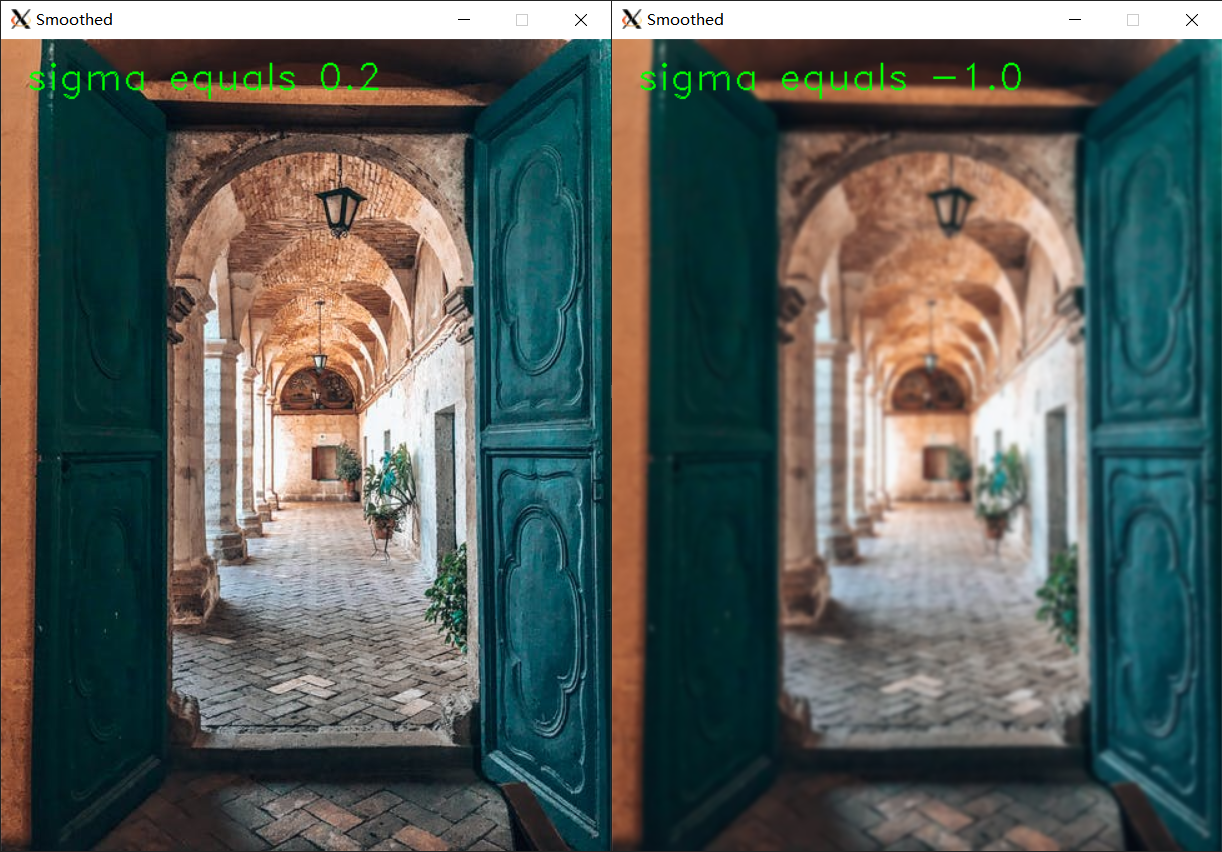
\includegraphics[width=0.8\textwidth]{assets/images/figures/std_dev.png}
   \caption{Blurring with different standard deviation}
   \label{fig:std_dev}
\end{figure}

Standard deviation, $\sigma$, dictates the width of the Gaussian distribution curve inside the kernel. The standard deviation equal to $0.2$ has a more concentrated distribution in the center than $-1$. Less centralized distribution gives blurrier image.

Note that the standard deviation cannot be negative. Here $-1$ is a valid value because it is squared in the formula.

\begin{equation*}
    G(x,y) = Ae^{-\frac{x^2+y^2}{2\sigma^2}}
\end{equation*}



\subsection{c}
\begin{figure}[htbp]
   \centering
   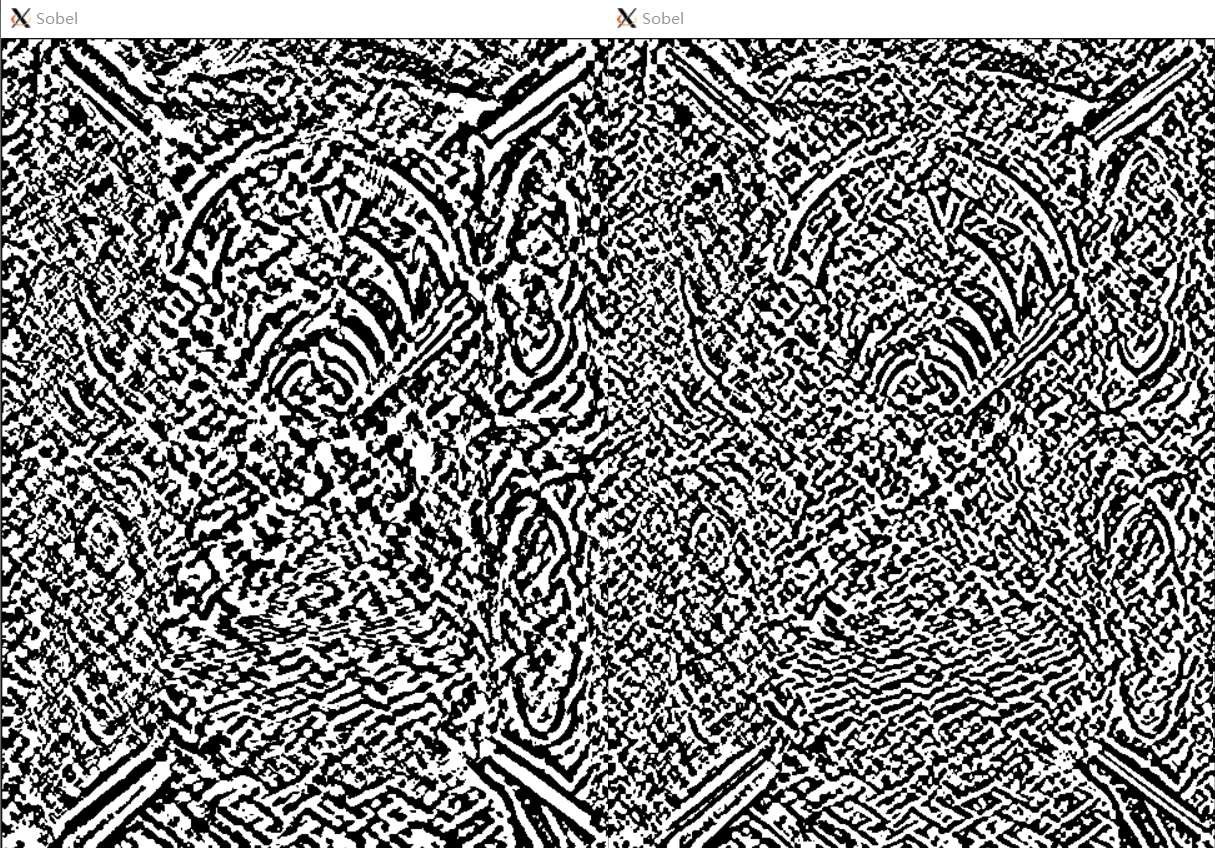
\includegraphics[width=0.8\textwidth]{assets/images/figures/Sobel_with_normalised_box_or_Gaussian.png}
   \caption{Sobel operator with normalised box filter (left), and with Gaussian filter (right)}
   \label{fig:Sobel_with_normalised_box_VS_with_Gaussian}
\end{figure}

Sobel operator with Gaussian smoothing gives more clear edges than with normalised box smoothing. This is because the box smoothing is not a low-pass filter so will cause high frequency artifacts \cite{ref:boxvsgaussian}. In other words, the box smoothing cannot produce clear edges. Thus, Gaussian smoothing is better for edge detection.



\subsection{d}
From observations, increasing the minimum threshold reduces decreases the amount of detected edges. The Canny edge detection algorithm is divided into four stage, the last stage is Hysteresis Thresholding \cite{ref:canny_ttl}. Hysteresis Thresholding decides which are really edges based on its intensity gradient calculated in the second stage or its connectivity. Possible edges with intensity gradient below the minimum threshold are discarded.

In addition, The larger the kernel size of Canny, the weaker the effect obtained by adjusting the minimum threshold by the same magnitude. This two parameters hold each other in check, allowing precise control of the amount of edges obtained.



\subsection{e}
After removing the blurring step which is the first stage of the Canny algorithm, many subtle edges are detected. This reflects the purpose of a smoothing; to remove the small noises and retain the important information. By blurring out the tiny edges in the image, it is more likely that the Canny edge detection yields only the edges of interest.



\subsection{f}
\begin{figure}[htbp]
   \centering
   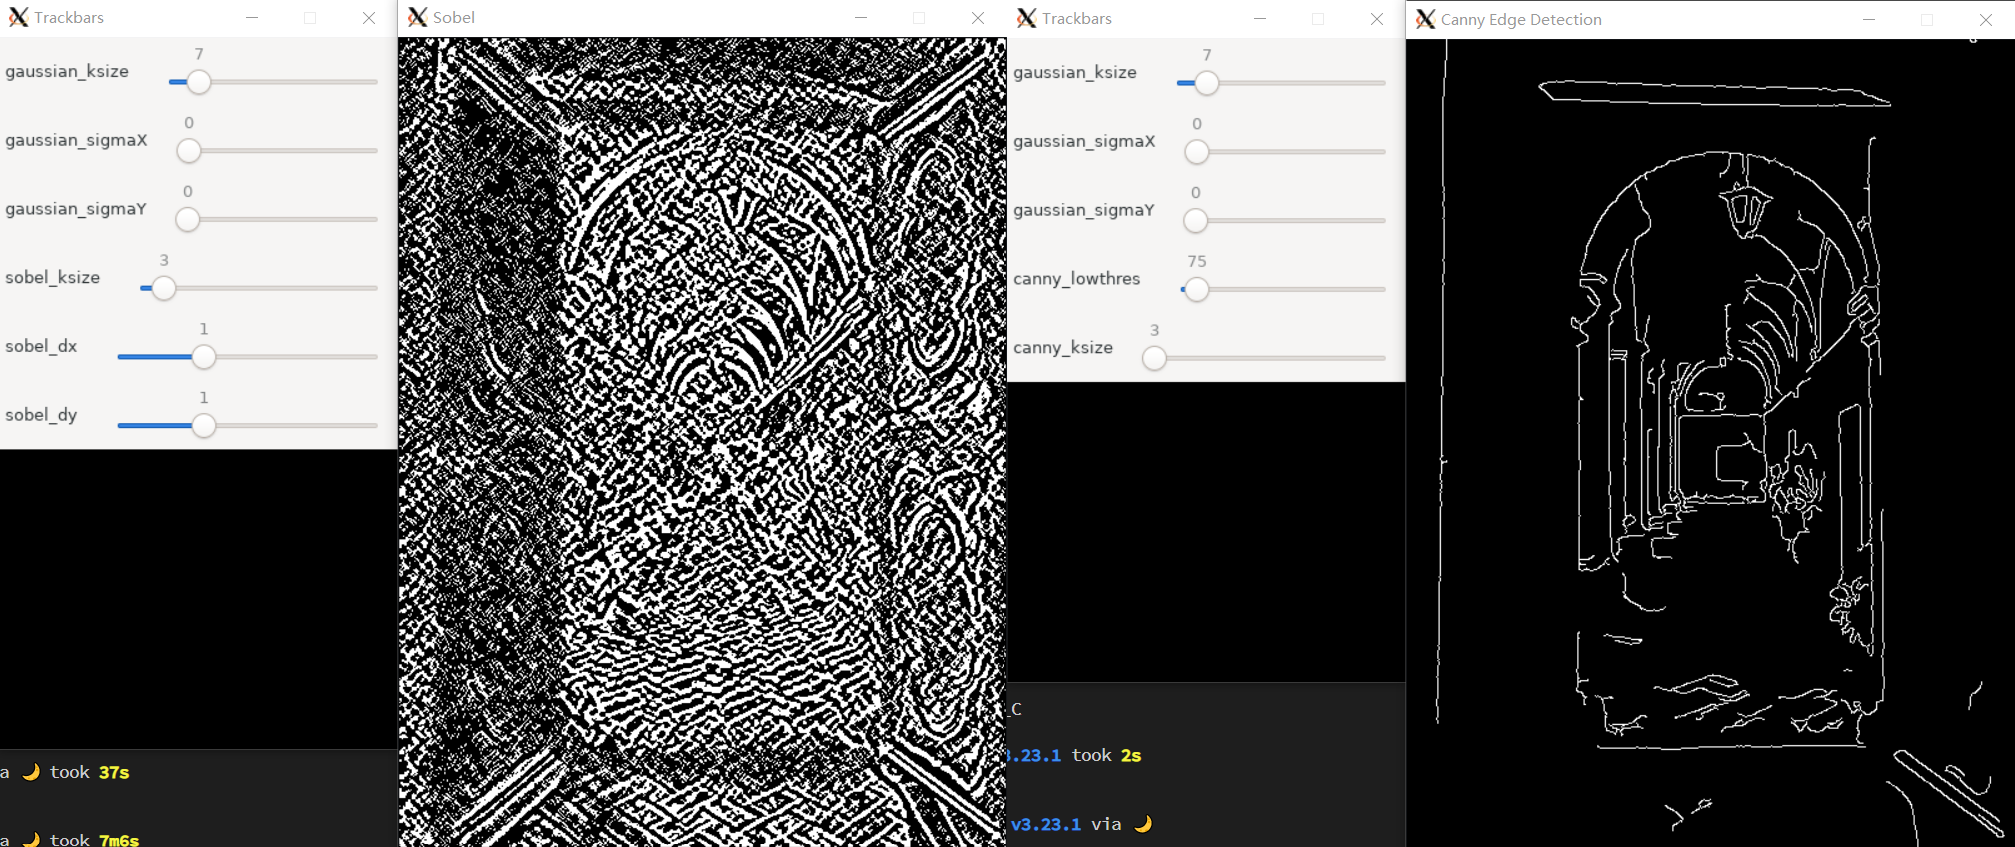
\includegraphics[width=\textwidth]{assets/images/figures/Sobel_VS_Canny.png}
   \caption{Sobel operator (left) versus Canny edge detection (right)}
   \label{fig:Sobel_VS_Canny}
\end{figure}

The Canny edge detection is built on top of the Sobel operator. Edges yields from Sobel operator are thick and contains noises. Moreover, Sobel operator cannot be controlled for getting wanted edges. The Canny edge detection further developed Sobel operator to solve these problems by adding three additional stages which are finding intensity gradient of the image, non-maximum suppression, and hysteresis thresholding \cite{ref:canny_ttl}. To be more specific, the non-maximum suppression yields thin edges, and the hysteresis thresholding extracts the edges of interest based on its intensity gradient and connectivity.



\subsection{g}
\begin{figure}[htbp]
   \centering
   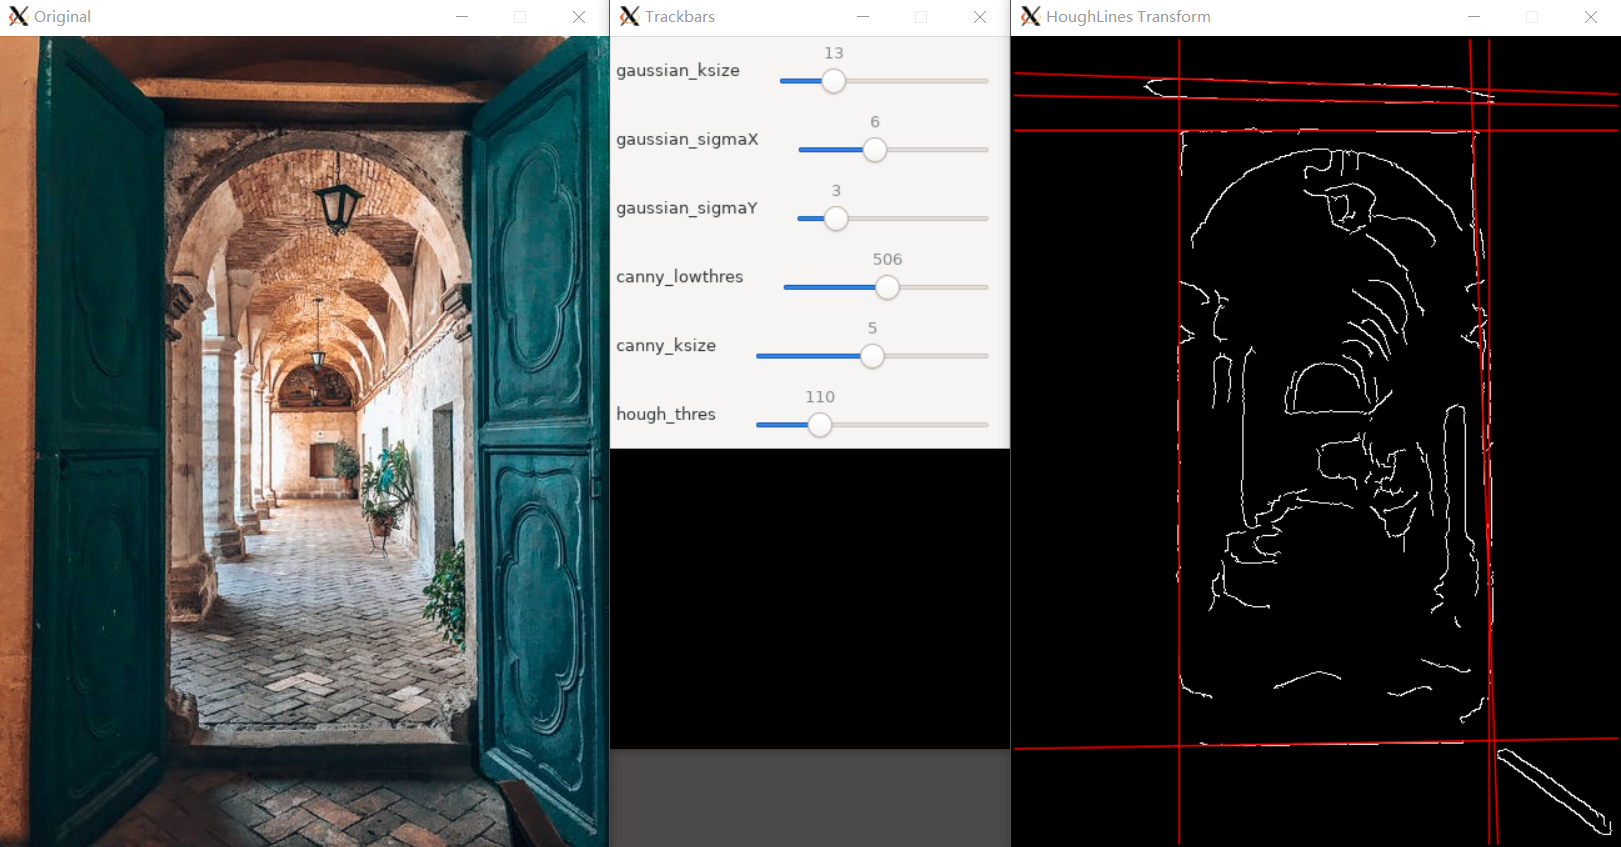
\includegraphics[width=0.9\textwidth]{assets/images/figures/edges_of_doorway.png}
   \caption{Edges of doorway}
   \label{fig:edges_of_doorway}
\end{figure}

The mobile robot can recognise the doorway and pass through it with the help of image processing. The red lines in Fig \ref{fig:edges_of_doorway} represent the straight edges of interest, which form the edges of a doorway. There are two redundant red lines at the top but does not matter.

The parameters shown in the middle of Fig \ref{fig:edges_of_doorway} are only for this image. The robot camera captures a stream of images split into frames. This means that the parameters should be different for each frame to extract the edges of doorway to ensure that the robot can pass. Dynamic thresholding is a solution for this situation.

\section{Part B Discussion}
The k-nearest neighbors (KNN) algorithm is a supervised machine learning method. It is a classic method for background subtraction.

It can be noticed that moving objects sometimes appear semi-transparent when using KNN. The explanation for this phenomenon is simple. KNN divides pixels into two categories: foreground and background. The category of a pixel can be represented by the neighbouring pixels. KNN incorrectly classifies some background pixels as foreground pixels, and because of the last sentence, a misclassification can infect the pixels around it, which results in blocks of background pixels appear on the moving objects.

Background subtraction can help robots to achieve target tracking and obstacle avoidance. Usually the target tracked is moving and by eliminating the background, the robot can better focus on the moving target. Robot obstacle avoidance is divided into two parts, one is avoiding static obstacles and the other is avoiding dynamic obstacles. Background subtraction helps the robot to identify potential dynamic obstacles. Generally speaking, background is usually a noise for robot applications because The primary purpose of giving robots vision is to identify living or moving things, and methods such as Lidar is enough for sensing background information. This type of noise can be eliminated gracefully thanks to the background subtraction algorithms.
